\chapter{Tools}

\section{Github} 
\label{def:github}
\label{def:githubDev}
It was requested by the customer that the group should use a version control system, with Github being preferable, to share code and perform version control. Github was used to share and synchronize code, and to describe and mark issues found in the code when problems were discovered. The relevant issues could then be discussed on the website.  Github is mostly used to update the followers of a repository and give them the newest version of the code, so it is  very ideal for coding in groups, where its users can simply push their finished work and the repository will automatically merge it with the already existing code, if done correctly.  Github has browser-based interfaces, download-able clients, and a robust command-line interface, meaning all the members of the group could make use of it. There were some problems associated with learning how to use and fix problems with it, as not all group members had experience with this tool, though other group members had heavy previous experience from other courses.

\section{Android Developer Tools Bundle}
An Integrated Development Environment(IDE) that fulfilled the following requirements was needed:
\begin{itemize}
\item Had to integrate support for Android Application Development.
\item Was able fairly easy to learn. 
\end{itemize}
The group decided to go with the Android Developer Tools Bundle, which essentially provided us with the Eclipse IDE and the Android Developer Tools. This bundle included everything needed to start developing an Android Application:
\begin{itemize}
\item Eclipse IDE + ADT plugin
\item Android SDK Tools
\item Android Platform-tools
\item The latest Android platform
\item The latest Android system image for the emulator
\end{itemize}

\section{Trello}  

Trello \label{def:trello} is a online collaboration tool with the ability to create interactive online boards. This helps any projects and groups to organize what is being worked on, who is working on what, and where in the progress some task is. Trello quickly became the most valuable tool to track the project tasks and progress, and to know who was working on which tasks. It simplified the group leaders task of maintaining control over project tasks a lot easier than it would have been without it. Shown in Figure \ref{img:trelloBoard} and Figure \ref{img:trelloCard} is an example of the Trello board, and a card representing a single task and sub-tasks. The board shows tasks sorted in several columns, according to priority and status. The card also includes information on which developers are assigned to the tasks, and how far the task has progressed. 
\begin{figure}
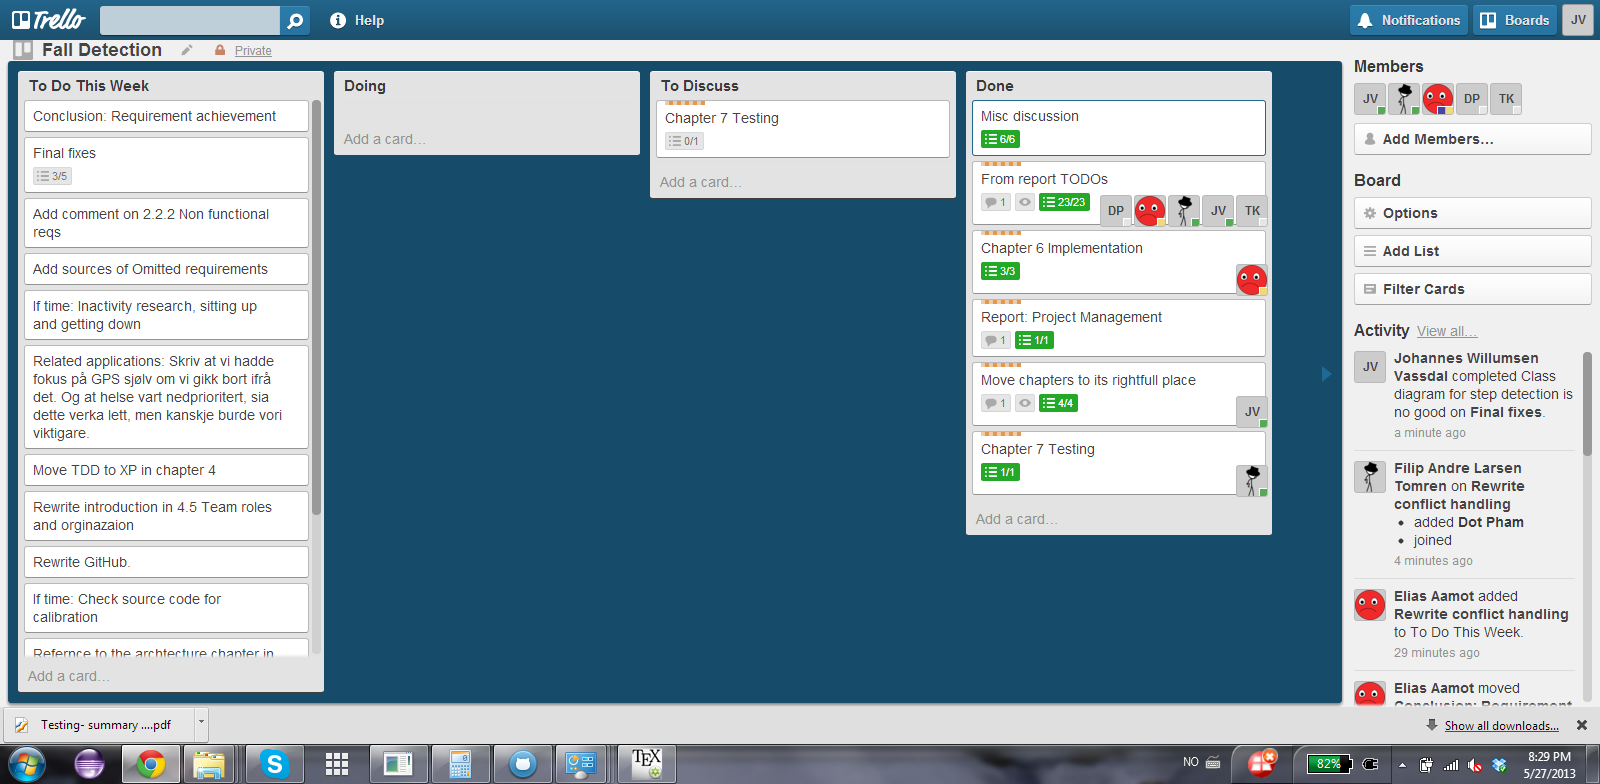
\includegraphics[width=\textwidth]{Res/TrelloBoard}
\caption{The Trello board}
\label{img:trelloBoard}
\end{figure}
\begin{figure}
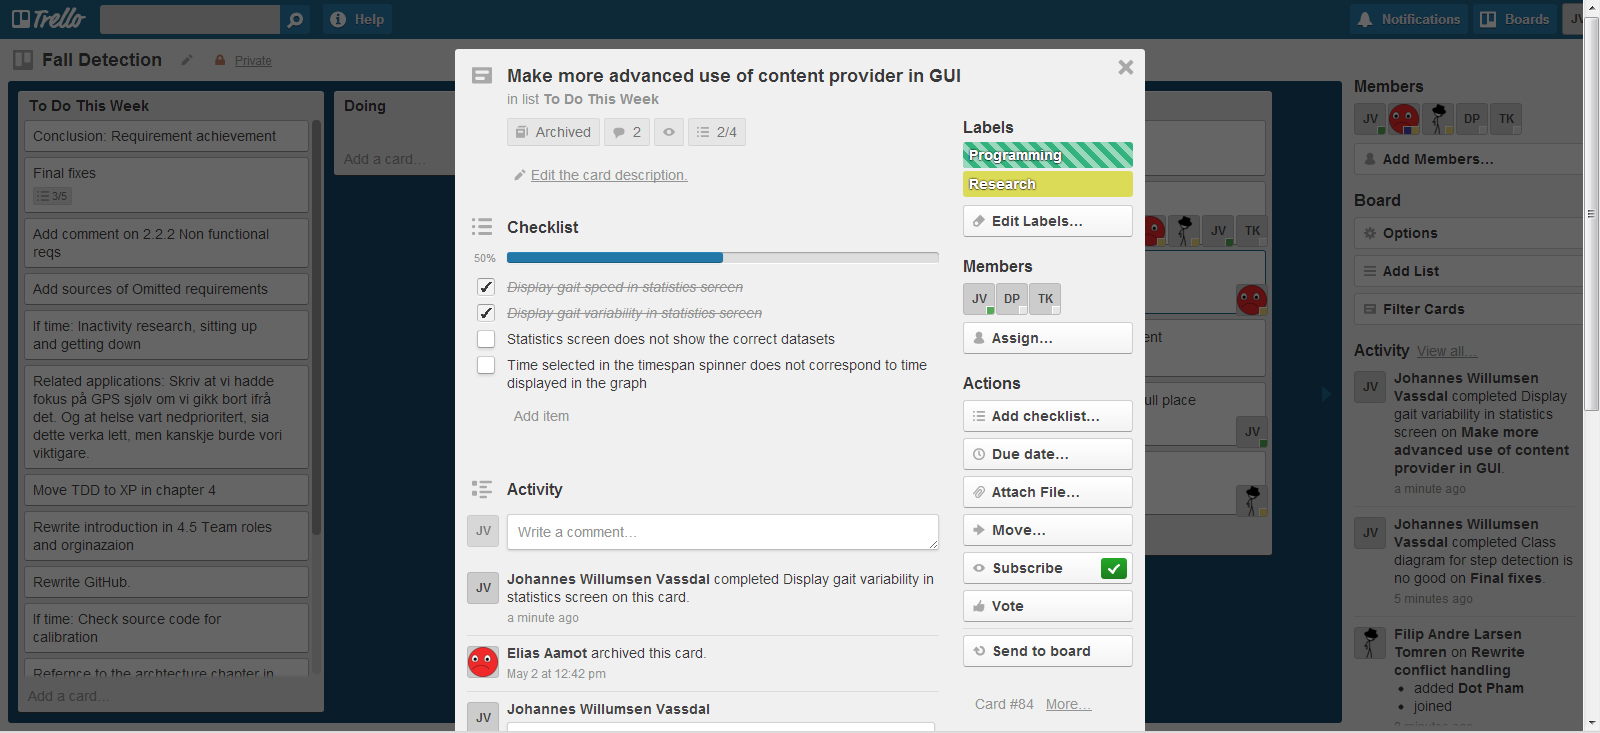
\includegraphics[width=\textwidth]{Res/TrelloCard}
\caption{Details on a Trello card, including checklist and people assigned}
\label{img:trelloCard}
\end{figure}


\section{itslearning}
Itslearning was used to distribute information that was not time -critical, with a message board being used. Itslearning would not send messages when a new topic or message appeared, so it's use for time critical messages or making sure that everyone would read it was limited. This also lead to it not being used as much as it should be the group, and its use quickly vanished.

\section{Email}
Email was used for time critical communication, and for information that needed feedback swiftly, often within the same day. It also became our main communication channel to distribute messages between members of the group.

\section{LaTeX}
\label{def:latex}
LaTeX was used to write this report. LaTeX is a typesetting language, with support for varied formatting, including images and including other documents. It also has the option allowed for inclusion of multiple LaTeX documents (.tex documents). This leads to improved readability of LaTeX code and increased productivity, as several chapters could be altered at the same time. This functionality allows a group of multiple users to avoid the problems associated with multiple users writing in the same document. The editor used was Texmaker, an free latex-editor available on multiple platforms.
